\newpage
\section{Durchführung}
    \subsection{Versuchsaufbau}

        \FloatBarrier

        \begin{figure}[h]
          \centering
          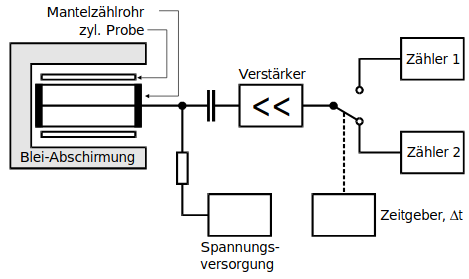
\includegraphics[width = 0.6\textwidth]{pictures/Aufbau.png}
          \caption{In der Abbildung ist eine schematische Darstellung der Zerfallskurve zweier Isotope, deren Halbwertszeiten stark verschieden sind. Die Anzahl der zerfallenden Kerne ist dabei logarithmisch gegen die Zeit aufgetragen. Die Zerfallskurve eines einzelnen Isotops würde linear verlaufen und das tun auch die linearen Regressionen der einzelnen Isotope (gestrichelt)  [1]}
          \label{fig:Aufbau}
        \end{figure}

        \FloatBarrier

        \noindent
        Wie im schematischen Aufbau zu erkennen, ist die Probe in einen Bleimantel gehüllt, um den Einfluss äußerer Strahlung auf die Messung zu verringern. Bei jedem zerfallenden Kern wird ein
        $\beta^-$-Teilchen freigesetzt, das auf dem Geiger-Müller-Zählrohr einen elektrischen Impuls erzeugt, der verstärkt und dann gemessenen wird. Ein Zeitschalter wechselt nach verstreichen
        des vorgewählten Zeitintervalls $\Delta t$ auf einen anderen Zähler, sodass ohne Unterbrechng zur Notierung der Daten weitergemessen werden kann.

    \subsection{Untergrundbestimmung}
        Trotz der Bleiummantelung ist ein Anteil an äußerer Strahlung vorhanden. Um diesen Huntergrund später abzuziehen, wird dieser zunächst bestimmt. Dazu werden Messungen ohne Probe im 
        Zählrohr mit einer Integrationszeit von 300 Sekunden durchgeführt.

    \subsection{Halbwertszeitbestimmung von Vanadium}
        Zur Halbwertszeitbestimmung von Vanadium wird eine Vanadiumprobe zunächst an einer Neutronenquelle platziert. Nachdem diese dort aktiviert wurde, wird sie in dem Zählrohr platziert und 
        die Aktivität über ein Messintervall von 30 Sekunden gemessen. Alle 30 Sekunden wechselt der Zeitschalter auf den anderen der zwei Zähler und ermöglicht so ein Ablesen der Zählrate auf
        dem anderen Zähler.

    \subsection{Halbwertszeitbestimmung von Rhodium}
        Die Rhodiumprobe wird entsprechend der Vorbereitung der Vanadiumprobe auch neben der Neutronenquelle aktiviert. Die Messung der Aktivität verläuft analog zur Messung der Vanadiumprobe
        mit einer Messzeit von 15 Sekunden. Auch hier ermöglicht der Zeitschalter ein kontinuierliches Messen.
        
